\section{Setup}\label{sc:setup}
To test our original scenario described in the Introduction on page \pageref{ch:introduction} we built a smaller version of the running track. To get a constant speed and track ew to run tests on we use a Brio\texttrademark train to symbolism a human runner that runs a track. The track we used in the teorie part was 400m but as to get something that would fit our test setup we caluated the scaling factor between the teori and the real track. We build two versions of the track a small one with the length of 43.5cm and a larger one having a length of 56cm. 


\begin{table}[H]
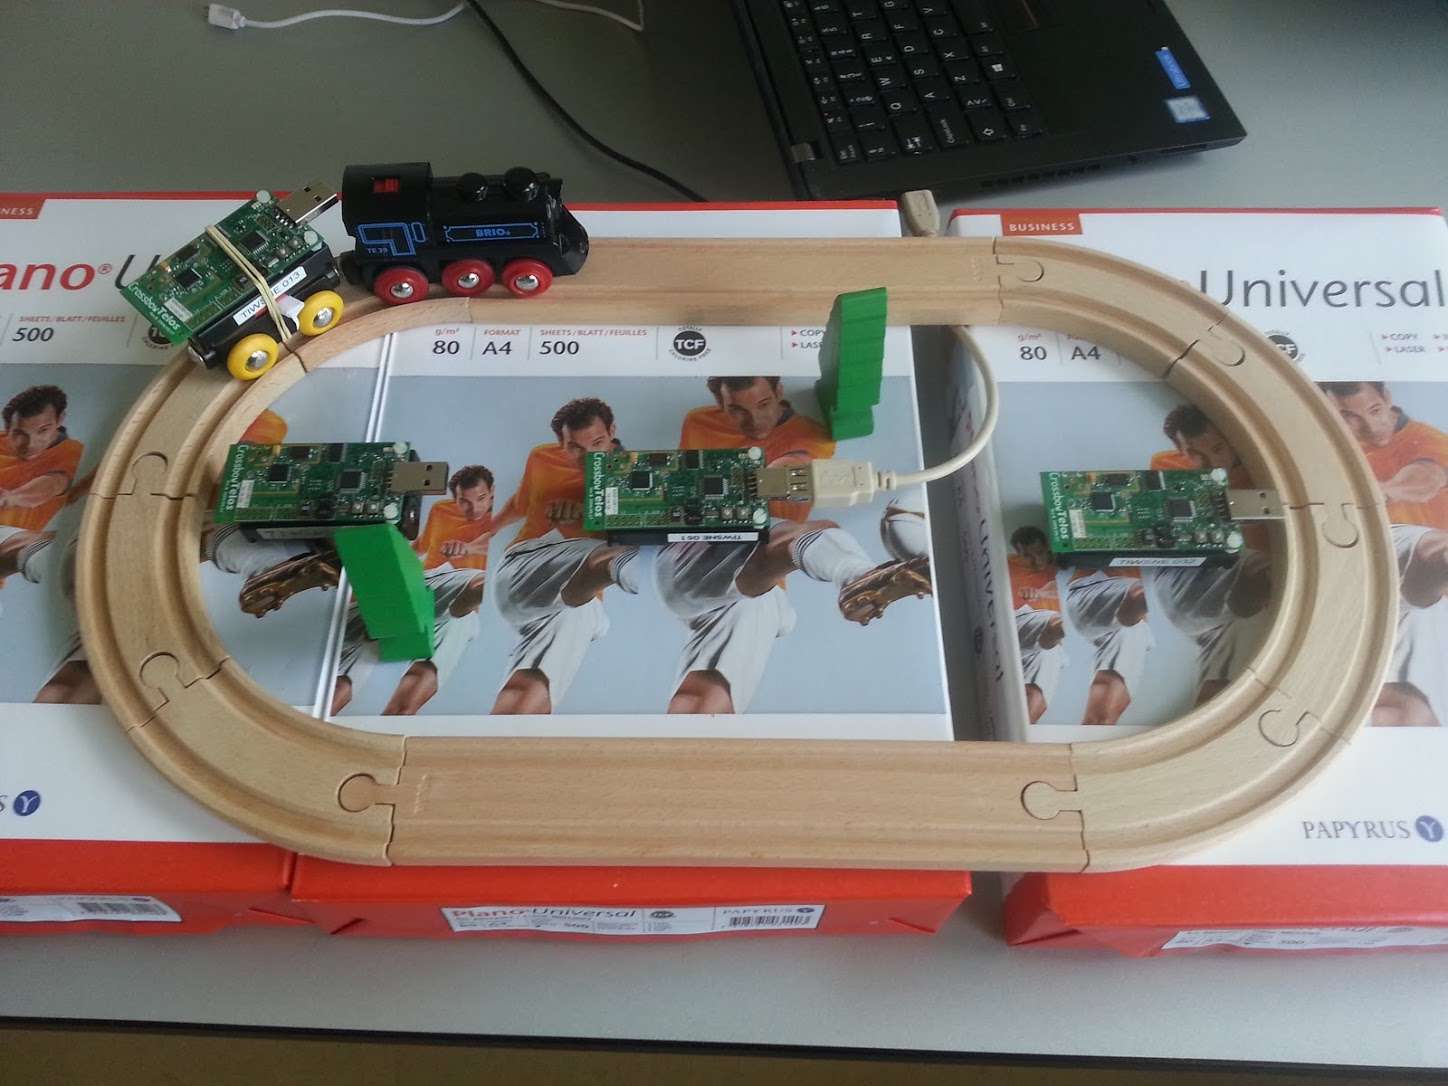
\includegraphics[width=1\linewidth]{testAndPerformance/setup/setup}\label{fig:testSetup}
\end{table}

